% Options for packages loaded elsewhere
% Options for packages loaded elsewhere
\PassOptionsToPackage{unicode}{hyperref}
\PassOptionsToPackage{hyphens}{url}
\PassOptionsToPackage{dvipsnames,svgnames,x11names}{xcolor}
%
\documentclass[
  british,
  a4paper,
]{article}
\usepackage{xcolor}
\usepackage{amsmath,amssymb}
\setcounter{secnumdepth}{-\maxdimen} % remove section numbering
\usepackage{iftex}
\ifPDFTeX
  \usepackage[T1]{fontenc}
  \usepackage[utf8]{inputenc}
  \usepackage{textcomp} % provide euro and other symbols
\else % if luatex or xetex
  \usepackage{unicode-math} % this also loads fontspec
  \defaultfontfeatures{Scale=MatchLowercase}
  \defaultfontfeatures[\rmfamily]{Ligatures=TeX,Scale=1}
\fi
\usepackage{lmodern}
\ifPDFTeX\else
  % xetex/luatex font selection
\fi
% Use upquote if available, for straight quotes in verbatim environments
\IfFileExists{upquote.sty}{\usepackage{upquote}}{}
\IfFileExists{microtype.sty}{% use microtype if available
  \usepackage[]{microtype}
  \UseMicrotypeSet[protrusion]{basicmath} % disable protrusion for tt fonts
}{}
\makeatletter
\@ifundefined{KOMAClassName}{% if non-KOMA class
  \IfFileExists{parskip.sty}{%
    \usepackage{parskip}
  }{% else
    \setlength{\parindent}{0pt}
    \setlength{\parskip}{6pt plus 2pt minus 1pt}}
}{% if KOMA class
  \KOMAoptions{parskip=half}}
\makeatother
% Make \paragraph and \subparagraph free-standing
\makeatletter
\ifx\paragraph\undefined\else
  \let\oldparagraph\paragraph
  \renewcommand{\paragraph}{
    \@ifstar
      \xxxParagraphStar
      \xxxParagraphNoStar
  }
  \newcommand{\xxxParagraphStar}[1]{\oldparagraph*{#1}\mbox{}}
  \newcommand{\xxxParagraphNoStar}[1]{\oldparagraph{#1}\mbox{}}
\fi
\ifx\subparagraph\undefined\else
  \let\oldsubparagraph\subparagraph
  \renewcommand{\subparagraph}{
    \@ifstar
      \xxxSubParagraphStar
      \xxxSubParagraphNoStar
  }
  \newcommand{\xxxSubParagraphStar}[1]{\oldsubparagraph*{#1}\mbox{}}
  \newcommand{\xxxSubParagraphNoStar}[1]{\oldsubparagraph{#1}\mbox{}}
\fi
\makeatother


\usepackage{longtable,booktabs,array}
\newcounter{none} % for unnumbered tables
\usepackage{calc} % for calculating minipage widths
% Correct order of tables after \paragraph or \subparagraph
\usepackage{etoolbox}
\makeatletter
\patchcmd\longtable{\par}{\if@noskipsec\mbox{}\fi\par}{}{}
\makeatother
% Allow footnotes in longtable head/foot
\IfFileExists{footnotehyper.sty}{\usepackage{footnotehyper}}{\usepackage{footnote}}
\makesavenoteenv{longtable}
\usepackage{graphicx}
\makeatletter
\newsavebox\pandoc@box
\newcommand*\pandocbounded[1]{% scales image to fit in text height/width
  \sbox\pandoc@box{#1}%
  \Gscale@div\@tempa{\textheight}{\dimexpr\ht\pandoc@box+\dp\pandoc@box\relax}%
  \Gscale@div\@tempb{\linewidth}{\wd\pandoc@box}%
  \ifdim\@tempb\p@<\@tempa\p@\let\@tempa\@tempb\fi% select the smaller of both
  \ifdim\@tempa\p@<\p@\scalebox{\@tempa}{\usebox\pandoc@box}%
  \else\usebox{\pandoc@box}%
  \fi%
}
% Set default figure placement to htbp
\def\fps@figure{htbp}
\makeatother



\ifLuaTeX
\usepackage[bidi=basic,shorthands=off]{babel}
\else
\usepackage[bidi=default,shorthands=off]{babel}
\fi
\ifLuaTeX
  \usepackage{selnolig} % disable illegal ligatures
\fi


\setlength{\emergencystretch}{3em} % prevent overfull lines

\providecommand{\tightlist}{%
  \setlength{\itemsep}{0pt}\setlength{\parskip}{0pt}}



 


\makeatletter
\@ifpackageloaded{tcolorbox}{}{\usepackage[skins,breakable]{tcolorbox}}
\@ifpackageloaded{fontawesome5}{}{\usepackage{fontawesome5}}
\definecolor{quarto-callout-color}{HTML}{909090}
\definecolor{quarto-callout-note-color}{HTML}{0758E5}
\definecolor{quarto-callout-important-color}{HTML}{CC1914}
\definecolor{quarto-callout-warning-color}{HTML}{EB9113}
\definecolor{quarto-callout-tip-color}{HTML}{00A047}
\definecolor{quarto-callout-caution-color}{HTML}{FC5300}
\definecolor{quarto-callout-color-frame}{HTML}{acacac}
\definecolor{quarto-callout-note-color-frame}{HTML}{4582ec}
\definecolor{quarto-callout-important-color-frame}{HTML}{d9534f}
\definecolor{quarto-callout-warning-color-frame}{HTML}{f0ad4e}
\definecolor{quarto-callout-tip-color-frame}{HTML}{02b875}
\definecolor{quarto-callout-caution-color-frame}{HTML}{fd7e14}
\makeatother
\makeatletter
\@ifpackageloaded{caption}{}{\usepackage{caption}}
\AtBeginDocument{%
\ifdefined\contentsname
  \renewcommand*\contentsname{Table of contents}
\else
  \newcommand\contentsname{Table of contents}
\fi
\ifdefined\listfigurename
  \renewcommand*\listfigurename{List of Figures}
\else
  \newcommand\listfigurename{List of Figures}
\fi
\ifdefined\listtablename
  \renewcommand*\listtablename{List of Tables}
\else
  \newcommand\listtablename{List of Tables}
\fi
\ifdefined\figurename
  \renewcommand*\figurename{Figure}
\else
  \newcommand\figurename{Figure}
\fi
\ifdefined\tablename
  \renewcommand*\tablename{Table}
\else
  \newcommand\tablename{Table}
\fi
}
\@ifpackageloaded{float}{}{\usepackage{float}}
\floatstyle{ruled}
\@ifundefined{c@chapter}{\newfloat{codelisting}{h}{lop}}{\newfloat{codelisting}{h}{lop}[chapter]}
\floatname{codelisting}{Listing}
\newcommand*\listoflistings{\listof{codelisting}{List of Listings}}
\makeatother
\makeatletter
\makeatother
\makeatletter
\@ifpackageloaded{caption}{}{\usepackage{caption}}
\@ifpackageloaded{subcaption}{}{\usepackage{subcaption}}
\makeatother
\usepackage{bookmark}
\IfFileExists{xurl.sty}{\usepackage{xurl}}{} % add URL line breaks if available
\urlstyle{same}
% fallback for those not using the hyperref driver hyperxmp:
\makeatletter
\@ifundefined{xmpquote}{\newcommand{\xmpquote}[1]{#1}}{}
\makeatother
\hypersetup{
  pdftitle={Making econometric results checkable},
  pdfauthor={Carlos Galindo},
  pdflang={en-GB},
  colorlinks=true,
  linkcolor={blue},
  filecolor={Maroon},
  citecolor={Blue},
  urlcolor={Blue},
  pdfcreator={LaTeX via pandoc}}


\title{Making econometric results checkable}
\usepackage{etoolbox}
\makeatletter
\providecommand{\subtitle}[1]{% add subtitle to \maketitle
  \apptocmd{\@title}{\par {\large #1 \par}}{}{}
}
\makeatother
\subtitle{Machine-written model code is checked against authoritative
references before it runs, and results are regenerated exactly from
stored inputs.}
\author{Carlos Galindo}
\date{}
\begin{document}
\maketitle


\begin{tcolorbox}[enhanced jigsaw, arc=.35mm, bottomrule=.15mm, breakable, colback=white, colframe=quarto-callout-note-color-frame, left=2mm, leftrule=.75mm, opacityback=0, rightrule=.15mm, toprule=.15mm]

\vspace{-3mm}\textbf{At a glance}\vspace{3mm}

\begin{itemize}
\tightlist
\item
  \textbf{Question.} How can an economist trust numbers produced with
  machine-generated model code, and later reproduce them?
\item
  \textbf{Approach.} Check every command against an authoritative
  reference before it runs; store inputs and raw diagnostics; regenerate
  results from those and compare them with the stored version; confirm
  the whole chain against a live run.
\item
  \textbf{Finding.} Regenerated diagnostics matched the stored version
  exactly for all seven series in the test case, and a fresh live run
  matched it again. A broad automatic check raised false alarms on
  correct code, so the checks were kept few and precise, each tied to a
  documented failure.
\item
  \textbf{Why it matters.} A table in a paper is only as good as the
  route that produced it. This makes the route inspectable.
\end{itemize}

\end{tcolorbox}

\subsection{The question}\label{the-question}

Econometric work is a chain: data, model specification, estimation, a
table of diagnostics, a paragraph of prose. Each link can fail without
any visible error. A mis-specified command can run and return numbers. A
diagnostic can be copied by hand from a screen. A paragraph can describe
a model more confidently than the output supports.

Machine-generated code makes this worse in one specific way. It is
fluent, so wrong syntax and invented commands look as plausible as
correct ones. The usual defence, reading the output and asking whether
it looks sensible, catches large errors and misses quiet ones.

The project asks two questions. Can code be checked against an
authoritative reference \emph{before} it runs, so that invented commands
never produce numbers? And can every reported result be regenerated
exactly from stored inputs, so that the table in a paper can be audited
rather than trusted?

\subsection{Approach}\label{approach}

The design has four layers, each answering a different failure.

\textbf{1. Reference-first generation.} An authoritative knowledge base
was built from the vendor documentation of the estimation environment: a
structured index of 335 commands (261 distinct names) with their syntax,
parameters, constraints and examples. Code is written from, and cited
to, that index instead of from memory. Every lookup returns the source
it came from.

\textbf{2. A deliberately small set of pre-run checks.} A second tool
checks scripts before they run. The first design was broad: flag any
command absent from the index. A viability probe killed it. On scripts
known to be correct it produced two to five false alarms per file, from
legitimate code the reference did not recognise and from gaps in the
reference itself. A rule that fires on good code teaches people to
ignore it. The checks were therefore rebuilt as a short list of precise
rules, each tied to a documented failure, each shipped with a synthetic
example that must trigger it, and each required to stay silent on the
whole library of known-good scripts.

\textbf{3. Stored inputs and regenerated results.} The raw diagnostic
output of each model-based seasonal-adjustment run is archived, then
parsed into structured records covering sample size, model orders,
residual tests, outliers and calendar effects. A formal schema rejects
records with unknown fields, wrong types or missing identifiers.
Re-parsing the archive reproduces the stored results with no live
software needed.

\textbf{4. End-to-end validation.} A parser can reproduce its own
earlier output and still be wrong. Two further checks address this.
Synthetic raw outputs with \emph{known} values test that extraction is
correct, independently of any stored result. And a live run on a real
workfile is compared with the stored record, so the stored record is
confirmed by an independent recomputation.

\subsection{What the work shows}\label{what-the-work-shows}

\textbf{Regeneration is exact.} Re-parsing the archive reproduced the
stored results exactly for all seven series in the price-correlation
study that the toolkit was built around. A fresh live run on one of
those series, from the workfile through estimation to parsed record,
then matched the stored record in full. The stored record was therefore
independently confirmed and not merely self-consistent. The figure below
shows the shape of that comparison with simulated numbers.

\begin{figure}

\centering{

\pandocbounded{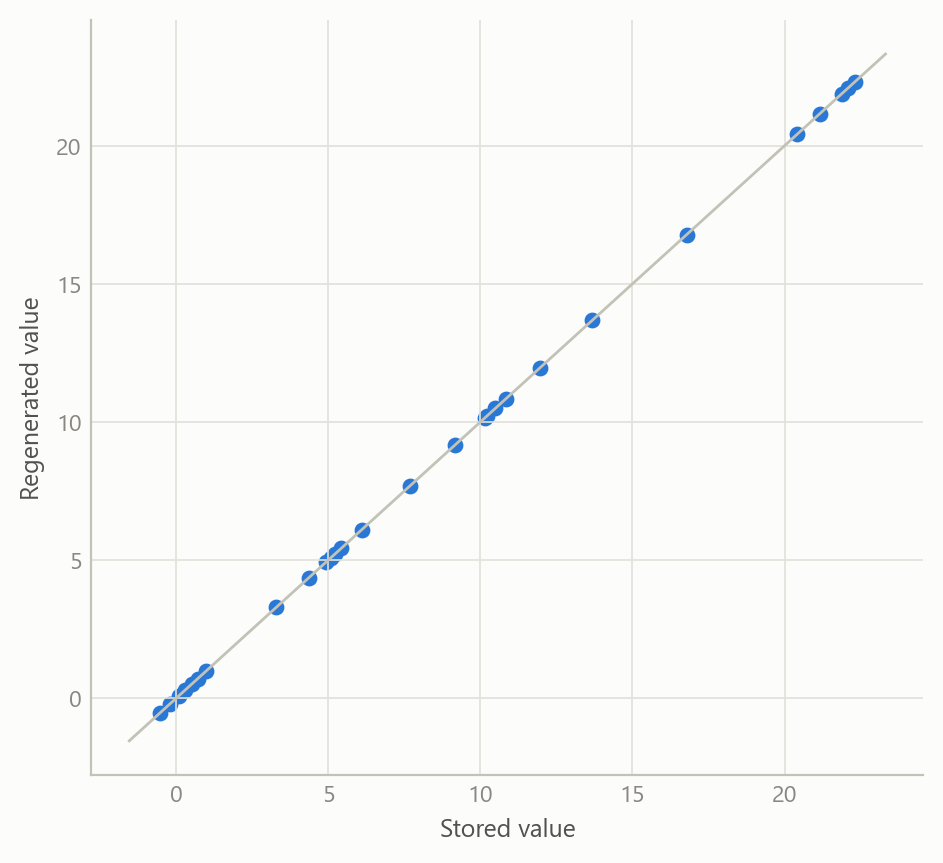
\includegraphics[keepaspectratio]{index_files/figure-latex/fig-regen-output-1.png}}

}

\caption{\label{fig-regen}Regenerated against stored diagnostics, seven
series and four statistics each (simulated data). Every point lies on
the 45-degree line: exact reproduction.}

\end{figure}%

\textbf{Broad checks fail; narrow checks work.} The probe on known-good
scripts is the clearest result. A rule that flags every unrecognised
command is noisy because no reference is complete. Curated rules, each
justified by a documented failure, produced no false alarms on the same
library. The figure illustrates the trade.

\begin{figure}

\centering{

\pandocbounded{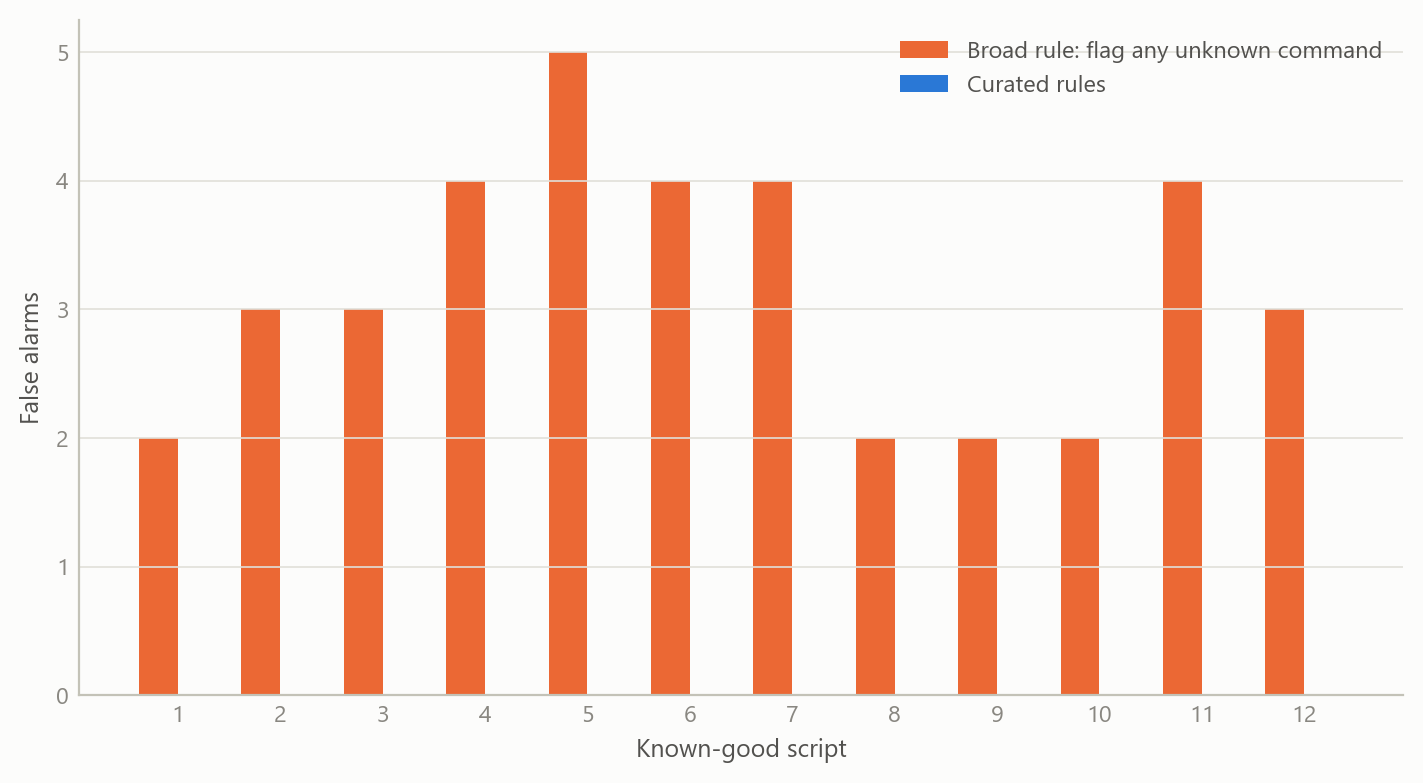
\includegraphics[keepaspectratio]{index_files/figure-latex/fig-checks-output-1.png}}

}

\caption{\label{fig-checks}False alarms per known-good script under two
checking designs (simulated data). The broad rule fires on correct code;
the curated rules stay silent.}

\end{figure}%

\textbf{Validation against many real runs corrected the project's own
prose.} The toolkit was checked against sixty-five archived runs of the
seasonal-adjustment procedure under different automation levels,
transformation choices and edge cases such as short samples and missing
values. All sixty-five parsed and passed the schema. They also exposed
an error in the project's own paper. Its text said a fixed seasonal
``airline'' model was imposed uniformly. In fact, at the lower
automation setting, the procedure still identifies the model, and some
series came out with richer orders. The mixed results were consistent
with the setting used; the sentence in the paper was imprecise. The
general claim that this setting imposes the airline model is not
universal.

\begin{figure}

\centering{

\pandocbounded{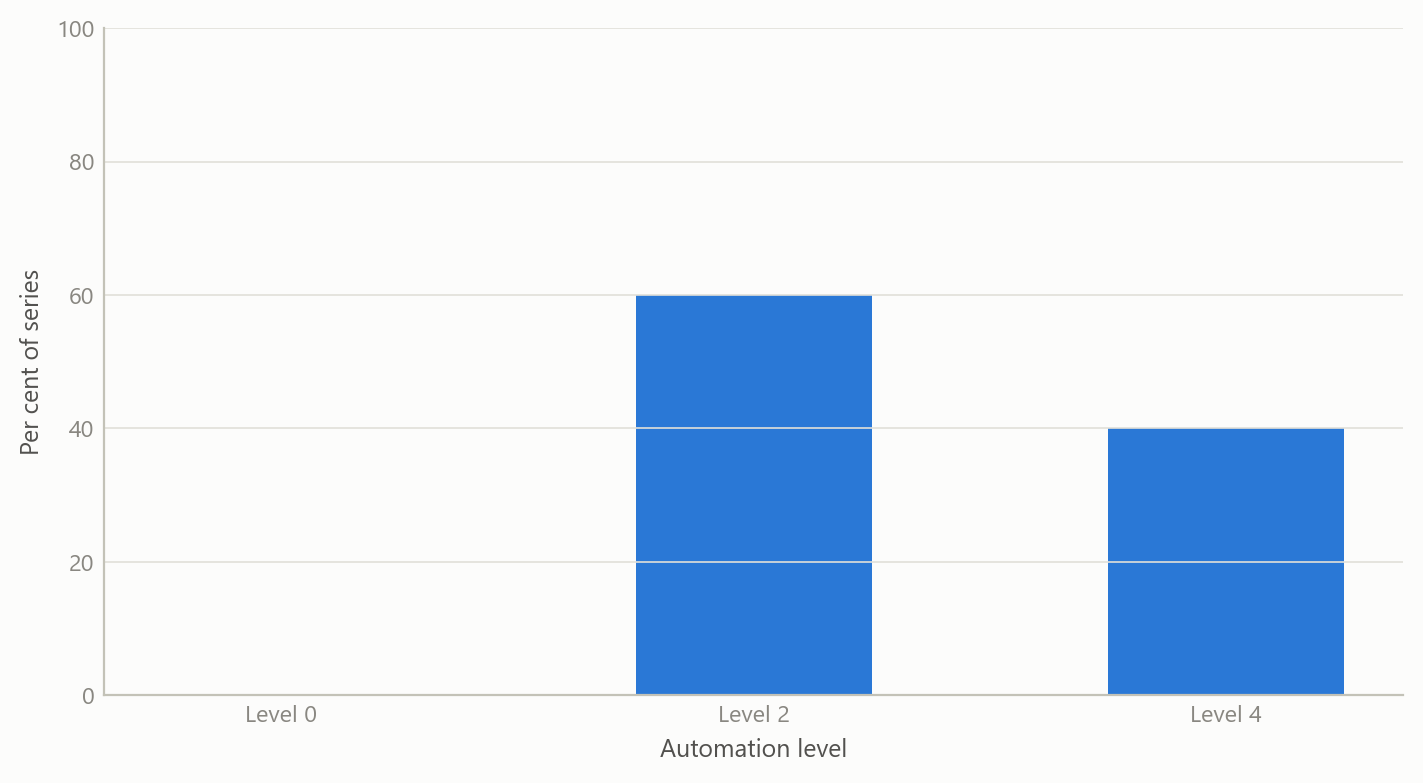
\includegraphics[keepaspectratio]{index_files/figure-latex/fig-models-output-1.png}}

}

\caption{\label{fig-models}Share of series with a non-airline model, by
automation level (simulated data, ten series per level). Levels that
still run model identification can return richer models.}

\end{figure}%

\subsection{Insights}\label{insights}

\begin{enumerate}
\def\labelenumi{\arabic{enumi}.}
\tightlist
\item
  \textbf{Matching your own earlier output is not correctness.}
  Reproducing a stored result shows a refactor preserved behaviour.
  Correctness needs a second source: known-value fixtures, and a live
  recomputation.
\item
  \textbf{Stand-in checks cannot find interface faults.} The live runs
  revealed faults in how results were retrieved that the stand-in tests
  were structurally unable to see. Where a tool talks to real software,
  a real run belongs in the test plan.
\item
  \textbf{Precision beats coverage in automatic checks.} A short rule
  list with a zero-false-alarm guarantee is used; a broad one is
  switched off. The honest outcome of the design review was to cut the
  proposed rule additions that could not meet that bar.
\item
  \textbf{Verification finds the author's own mistakes.} The sharpest
  finding was an overstatement in a draft paper, caught because the
  numbers had been regenerated rather than recalled.
\item
  \textbf{Cite the source of every answer.} Returning the reference
  alongside each lookup turns ``the machine said so'' into something a
  reader can check.
\end{enumerate}

\subsection{Limits and next steps}\label{limits-and-next-steps}

The checks cover a small set of documented traps. It cannot judge
whether a model is appropriate, and some real errors, such as claiming
model identification at a setting that does not perform it, depend on
intent and cannot be found by reading code. The reference index covers
the commands extracted so far, not the full language. Some components
have so far been validated only on crafted cases, and everything has
been run in a single computing environment, so portability is unproven.

Next steps are a wider set of crafted raw outputs, validation of the
second connection route, and extending the same regenerate-and-compare
discipline from seasonal-adjustment diagnostics to estimated model
coefficients and forecasts.

\subsection{About the evidence}\label{about-the-evidence}

The work was done in 2025--2026 during a career break and draws on a
documented reference index, an archived set of model runs, and the
validation record of the tools. The figures on this page are simulated
to show structure only; counts and findings in the text come from the
project's own records.

Figures and tables marked \emph{simulated} are generated from simulated
data built to share the structure of the analysis (its variables,
horizons and frequencies). They show how the method works and what its
output looks like; they are not the project's results. Results stated in
the text are the project's own. Methods are described at the level of a
methods section. Code and data pipelines are not reproduced here.




\end{document}
